\section{Durchführung}
\label{sec:Durchführung}
Der Aufbau ist in Abbildung \ref{fig:spek} dargestellt.
\begin{figure}[H]
  \centering
  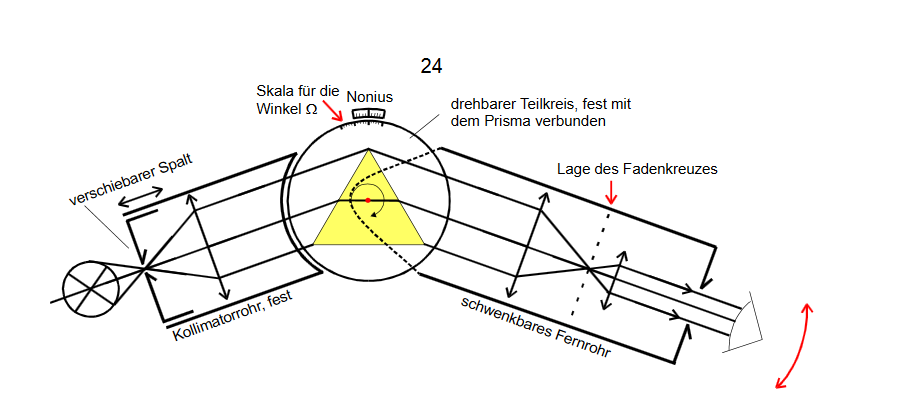
\includegraphics[scale=0.5]{content/pris_spek.png}
  \caption{Schematische Darstellung eines Prismen-Spektralapparats\cite{v402}.}
  \label{fig:spek}
\end{figure}
\noindent Am Ende des Kollimatorrohrs befindet sich eine Leuchtquelle.
Das Licht, welches von dieser ausgeht, fällt durch einen Spalt und eine Sammellinse auf ein Glasprisma und wird dort gebrochen.
Nach seiner Brechung gelangt das Licht in ein Fernrohr.
Die Objektivlinse entwirft ein reeles Spaltbild in ihrer Brennebene.
Zur genauen lokalisierung des Spaltbildes ist dort ein Fadenkreuz aufgetragen.
Durch schwenken um die Goniometerachse kann dann das Faenkreuz mit dem Spaltbild zur Deckung gebracht werden.
\subsection{Bestimmung der Richtungsänderung des Strahls}
Der $\eta$-Winkel beschreibt die Richtungsänderung des einfallenden Strahls.
Der Strahlengang von dem gebrochenen und dem reflektiertem Strahl sollen parallel verlaufen.
Dies kann realisiert werden, wenn das Prisma gleichschenklig ist und der Strahlengang symmetrisch ist.
Damit ein symmetrischer Strahlengang gefunden werden kann, wird das Prisma so lange um die Goniometerachse geschwenkt bis das reflektierte Spaltbild mit dem gebrochenen übereinstimmt.
Mit dem reflektiertem Spaltbild werden so die Spektrallinien der Lichtquelle abgefahren.
Dabei wird die Winkelstellung des Fernrohrs als auch die Farbe der Spektrallinie notiert.
Danach wird die Messung bei Spiegelsymmetrischer Stellung des Prismas wiederholt.
Die erforderliche Prismenstellung ist in Abbildung \ref{fig:eta} schematisch dargestellt.
\begin{figure}[H]
  \centering
  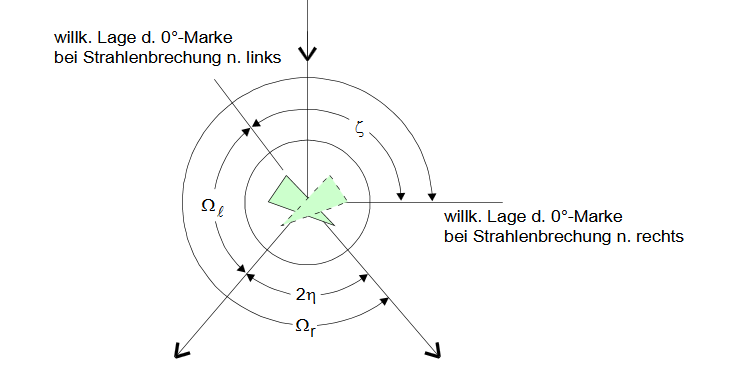
\includegraphics[scale= 0.5]{content/eta.png}
  \caption{Darstellung der Messgrößen $\Omega_l$ und $\Omega_r$ in Abbhängigkeit der Prismenstellungen\cite{v402}.}
  \label{fig:spek}
\end{figure}
\noindent Der Winkel $\eta$ kann dann mit
\begin{equation}
  \label{eq:eta}
  \eta = 180 -(\Omega_r - \Omega_l)
\end{equation}
bestimmt werden.
\subsection{Bestimmung des Brechungswinkels}
Das Prisma wird mit seiner brechenden Kante auf das Kollimatorrohr ausgerichtet.
Das Licht wird an der Prismenoberfläche reflektiert.
Die Reflektionswinkel, dargestellt in Abbildung \ref{fig:phi}, werden mit dem Fernrohr bestimmt.
\begin{figure}[H]
  \centering
  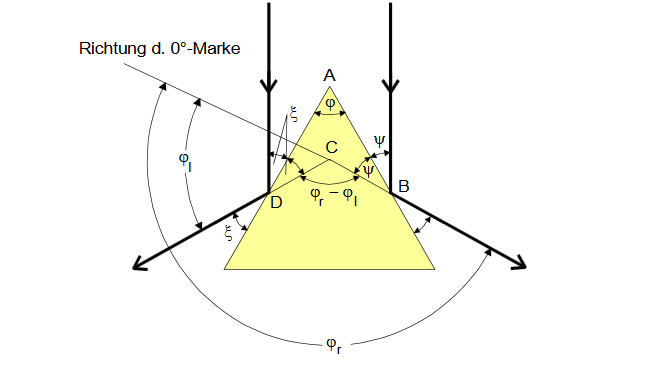
\includegraphics[scale=0.5]{content/phi.png}
  \caption{Skizze zur Bestimmung des Winkels $\phi$ zwischen den brechenden Oberflächen\cite{v402}.}
  \label{fig:phi}
\end{figure}
\noindent Die Messung wird für sechs verschiedene Prismenstellungen wiederholt.
Der Brechungswinkel $\phi$ kann dann wie folgt berechnet werden:
\begin{equation}
  \label{eq:phi}
  \varphi = \frac{1}{2}(\varphi_r -\varphi_l) .
\end{equation}
